% ---------------------------------------------------------------------------------------------------------------
% TEMPLATE PARA PROPOSTA DE TRABALHO DE CONCLUSÃO DE CURSO
% Universidade Tecnológica Federal do Paraná - UTFPR
% Customização da classe abnTeX2 (http://www.abntex.net.br/) para as normas da UTFPR
%
% Projeto: http://tcc.tsi.gp.utfpr.edu.br/paginas/modelos-latex-da-utfpr
% Autores: Diego Marczal
% 	   Michael Vornes <https://github.com/mvornes>
%
%----------------------------------------------------------------------------------------------------------------
% Codificação: UTF-8
% LaTeX:  abnTeX2
% ---------------------------------------------------------------------------------------------------------------


% CARREGA CLASSE PERSONALIZADA DA UTFPR--------------------------------------------------------------------------
\documentclass[%twoside,                   % Impressão em frente e verso
    	        oneside,                   % Impressão apenas frente
]{configuracoes/utfpr-abntex2}


% INCLUI ARQUIVOS DE CONFIGURAÇÕES-------------------------------------------------------------------------------
% REFERÊNCIAS------------------------------------------------------------------
\usepackage[%
    alf,
    abnt-emphasize=bf,
    bibjustif,
    recuo=0cm,
    abnt-url-package=url,       % Utiliza o pacote url
    abnt-refinfo=yes,           % Utiliza o estilo bibliográfico abnt-refinfo
    abnt-etal-cite=3,
    abnt-etal-list=3,
    abnt-thesis-year=final
]{abntex2cite}                  % Configura as citações bibliográficas conforme a norma ABNT

% PACOTES----------------------------------------------------------------------
\usepackage[utf8]{inputenc}                                 % Codificação do documento
%\usepackage[portuguese]{babel}								% Inserido por mim, por conta da cedilha
\usepackage[T1]{fontenc}                                    % Seleção de código de fonte
\usepackage{booktabs}                                       % Réguas horizontais em tabelas
\usepackage{color, colortbl}                                % Controle das cores
\usepackage{float}                                          % Necessário para tabelas/figuras em ambiente multi-colunas
\usepackage{graphicx}                                       % Inclusão de gráficos e figuras
\usepackage{icomma}                                         % Uso de vírgulas em expressões matemáticas
\usepackage{indentfirst}                                    % Indenta o primeiro parágrafo de cada seção
\usepackage{microtype}                                      % Melhora a justificação do documento
\usepackage{multirow, array}                                % Permite tabelas com múltiplas linhas e colunas
\usepackage{subeqnarray}                                    % Permite subnumeração de equações
\usepackage{lastpage}                                       % Para encontrar última página do documento
\usepackage{verbatim}                                       % Permite apresentar texto tal como escrito no documento, ainda que sejam comandos Latex
\usepackage{amsfonts, amssymb, amsmath}                     % Fontes e símbolos matemáticos
\usepackage[algoruled, portuguese]{algorithm2e}             % Permite escrever algoritmos em português
%\usepackage[scaled]{helvet}                                % Usa a fonte Helvetica
\usepackage{times}                                          % Usa a fonte Times
%\usepackage{palatino}                                      % Usa a fonte Palatino
%\usepackage{lmodern}                                       % Usa a fonte Latin Modern
\usepackage[bottom]{footmisc}                               % Mantém as notas de rodapé sempre na mesma posição
\usepackage{ae, aecompl}                                    % Fontes de alta qualidade
\usepackage{latexsym}                                       % Símbolos matemáticos
\usepackage{lscape}                                         % Permite páginas em modo "paisagem"
%\usepackage{picinpar}                                      % Dispor imagens em parágrafos
%\usepackage{scalefnt}                                      % Permite redimensionar tamanho da fonte
%\usepackage{subfig}                                        % Posicionamento de figuras
\usepackage{upgreek}                                       % Fonte letras gregas

% Redefine a fonte para uma fonte similar a Arial (fonte Helvetica)
\renewcommand*\familydefault{\sfdefault}

% CONFIGURAÇÕES DE APARÊNCIA DO PDF FINAL---------------------------------------
\makeatletter
\hypersetup{%
    portuguese,
    colorlinks=true,   % true: "links" coloridos; false: "links" em caixas de texto
    linkcolor=blue,    % Define cor dos "links" internos
    citecolor=blue,    % Define cor dos "links" para as referências bibliográficas
    filecolor=blue,    % Define cor dos "links" para arquivos
    urlcolor=blue,     % Define a cor dos "hiperlinks"
    breaklinks=true,
    pdftitle={\@title},
    pdfauthor={\@author},
    pdfkeywords={abnt, latex, abntex, abntex2}
}
\makeatother

% ALTERA O ASPECTO DA COR AZUL--------------------------------------------------
\definecolor{blue}{RGB}{41,5,195}

% REDEFINIÇÃO DE LABELS---------------------------------------------------------
\renewcommand{\algorithmautorefname}{Algoritmo}
\def\equationautorefname~#1\null{Equa\c c\~ao~(#1)\null}

% CRIA ÍNDICE REMISSIVO---------------------------------------------------------
\makeindex

% HIFENIZAÇÃO DE PALAVRAS QUE NÃO ESTÃO NO DICIONÁRIO---------------------------
\hyphenation{%
    qua-dros-cha-ve
    Kat-sa-gge-los
}

% CENTRALIZAR CONTEÚDO DA CÉLULA USANDO M
\newcolumntype{M}[1]{>{\centering\arraybackslash}m{#1}}



% INCLUI ARQUIVOS DA PROPOSTA DE TRABALHO DE CONCLUSÃO DE CURSO (PRÉ-TEXTUAIS, TEXTUAIS, PÓS-TEXTUAIS)------------

% INSERE CAPA E FOLHA DE ROSTO
% CAPA---------------------------------------------------------------------------------------------------

% DADOS DO TRABALHO--------------------------------------------------------------------------------------
\titulo{Processamento de Linguagem Natural Aplicada a Textos Jurídicos}
\autor{Daniel Elias dos Santos}
\autorcitacao{ELIAS, Daniel} % Sobrenome em maiúsculo
\local{Sabará}
\data{2019}

% NATUREZA DO TRABALHO-----------------------------------------------------------------------------------
\projeto{Pré-Projeto de Trabalho de Conclusão de Curso}

% TÍTULO ACADÊMICO---------------------------------------------------------------------------------------
% - Bacharel
\tituloAcademico{Bacharel}

% DADOS DA INSTITUIÇÃO-----------------------------------------------------------------------------------
% Coloque o nome do curso de graduação em "programa"
% Formato para o logo da Instituição: \logoinstituicao{<escala>}{<caminho/nome do arquivo>}
\instituicao{Instituto Federal de Educação, Ciência e Tecnologia de Minas Gerais}
\departamento{}
\programa{Curso de Bacharelado em Sistemas de Informação}
\logoinstituicao{0.2}{dados/figuras/logo-instituicao.jpg} 

% DADOS DOS ORIENTADORES---------------------------------------------------------------------------------
\orientador{Daniel Bruno Fernandes Conrado}
%\orientador[Orientadora:]{Nome da orientadora}
\instOrientador{}

%\coorientador{}
\coorientador[Coorientadora:]{Cristiane Norbiato Targa}
\instCoorientador{}

% FOLHA DE ROSTO--------------------------------------------------------------------------------------------------------

% TRABALHO DE CONCLUSÃO DE CURSO
 \preambulo{{\imprimirprojeto} de graduação, apresentado ao curso de {\imprimirprograma}, do {\imprimirinstituicao}, como requisito parcial para a obtenção do título de {\imprimirtituloAcademico}.}

% OBSERVAÇÕES-----------------------------------------------------------------------------------------------------------
% Este arquivo não precisa ser alterado.


\begin{document}
% INSERE ELEMENTOS PRÉ-TEXTUAIS
\pretextual
\imprimircapa                                               	           % Comando para imprimir Capa
\imprimirfolhaderosto{}                                     		   % Comando para imprimir Folha de rosto

\textual
% INSERE ELEMENTOS TEXTUAIS
% PROPOSTA DE TRABALHO DE CONCLUSÃO DE CURSO-----------------------------------------------------------

\chapter{PROPOSTA DE TRABALHO DE CONCLUSÃO DE CURSO}
\label{chap:proposta}

\section{TÍTULO}
\label{sec:titulo}
% Informe o título do trabalho-------------------------------------------------------------------------
%------------------------------------------------------------------------------------------------------
\thetitle.

\section{MODALIDADE DO TRABALHO}
\label{sec:modalidade}
% Indique a Modalidade do Trabalho---------------------------------------------------------------------
% Opções:
% - Pesquisa
% - Desenvolvimento de Sistemas
Pesquisa e Desenvolvimento de Sistemas
%------------------------------------------------------------------------------------------------------

\section{ÁREA DO TRABALHO}
\label{sec:area}
% Indique a Área do Trabalho---------------------------------------------------------------------------
Ciência de dados.
%------------------------------------------------------------------------------------------------------

\section{RESUMO}
\label{sec:resumo}
% Resumo do Trabalho-----------------------------------------------------------------------------------
% (máximo de 200 palavras)
Métodos tradicionais de mapeamento de hotspots, como a Estimativa de Densidade por Kernel (KDE) estática, são insuficientes para analisar fenômenos criminais dinâmicos, pois ocultam a evolução dos padrões no tempo e espaço. Este trabalho tem o objetivo de desenvolver e validar uma metodologia computacional automatizada para a análise espaço-temporal dinâmica de hotspots de furto de cabos, a fim de aprimorar a atividade de monitoramento do Centro Integrado de Operações da Prefeitura de Belo Horizonte (COP-BH). A metodologia proposta, aplicada sobre um dataset real, segmenta a análise em janelas temporais para identificar clusters com significância estatística. A validação será realizada por meio da comparação do novo método com a abordagem atualmente utilizada, através do Índice de Acurácia Preditiva (PAI). A partir disso pretende-se identificar o surgimento, dissipação e deslocamento dos hotspots, padrões que a análise estática não detecta. Espera-se que a metodologia ofereça uma ferramenta de inteligência mais eficaz para as ações de monitoramento, permitindo uma alocação eficiente de recursos, além de estabelecer uma base técnica robusta para aplicações futuras, como a ativação seletiva de analíticos de vídeo para prevenção.

Palavras-chave: Análise de dados, Mapeamento de Hotspots, Análise Espaço-Temporal, Ações Baseadas em Evidências, Furto de Cabos.

%------------------------------------------------------------------------------------------------------

                               % Proposta de TCC
% DESCRIÇÃO DA PROPOSTA--------------------------------------------------------------------

\chapter{DESCRIÇÃO DA PROPOSTA}
\label{chap:descricao}

\section{INTRODUÇÃO}
\label{sec:introducao}
% Introdução-------------------------------------------------------------------------------
O Centro Integrado de Operações da Prefeitura de Belo Horizonte (COP-BH), é a entidade municipal responsável pela integração de informações e da atuação das Instituições envolvidas na resposta a problemas públicos de Belo Horizonte. Suas atividades se baseiam no \textit{Modelo de Gestão Integrada do COP-BH} \cite{ModeloGestaoCOP}, que expressa o seu posicionamento institucional e como promove a integração, alinhamento e harmonização dos processos de trabalho de diversas Instituições e Agências comprometidas com o cuidado da cidade.

Pode ser classificado, segundo a Carta Brasileira para Cidades Inteligentes \cite{CartaCidades}, como um ``Centro de Gestão Integrada - GCI'', sendo este um ambiente estratégico que busca melhorar a eficiência e eficácia da prestação de serviços públicos ao aprimorar a proteção social e governança pública.

O COP-BH viabiliza a integração entre as Instituições e Agências por meio de seis linhas de atuação: \textit{Monitoramento da Cidade, Pronta Resposta, Gestão de Crises, Operações Integradas, Gestão de Eventos e Prevenção de Problemas.}

Conforme o citado modelo \cite{ModeloGestaoCOP}, a linha de atuação de Monitoramento da Cidade possui três vertentes: o monitoramento de sensores não especialistas, tais como câmeras, o monitoramento de sensores especialistas, tais como os meteorológicos, e o monitoramento de fontes de inteligência. Seu objetivo final é permitir que o COP-BH aja preventivamente a fim de evitar problemas públicos ou responder adequadamente a estes, minorando as suas consequências.

Este trabalho analisa e propõe uma mudança no método de análise de dados, bem como sua automatização, para suporte a uma das atividades da linha de atuação de Monitoramento da Cidade, relacionadas ao monitoramento de câmeras, que se delinea a seguir.

\subsection{Contextualização do Projeto}

Conforme descreve o modelo \cite{ModeloGestaoCOP}, a atividade de monitoramento se utiliza de diversos tipos de sensores para sua consecução. Dentre estes sensores, as câmeras instaladas em locais públicos permitem acesso à visualização de diversos pontos da cidade em tempo real.

A atividade de monitoramento das câmeras, ou seja, a visualização das suas imagens em tempo real, é realizada por agentes das Instituições que têm assento no ambiente chamado Sala de Controle Integrado, local onde as imagens são acessadas com o propósito de identificar problemas públicos mais rapidamente, a fim de possibilitar maior celeridade também à resposta.

São diversos os tipos de problemas públicos monitorados, tais como a deposição clandestina de lixo ou inservíveis em locais impróprios, animais de grande porte soltos em via pública, pichação, depredação, acidentes de trânsito, invasão de áreas protegidas e furtos de cabos, entre outros.

Para tornar o serviço mais eficiente, o COP-BH desenvolveu um processo de análise de dados sobre problemas públicos para elaborar um roteiro de monitoramento, que sugere os problemas que devem ser monitorados, os períodos de maior relevância para executar o monitoramento e quais as câmeras deveriam ser monitoradas. 

A partir deste roteiro, as equipes de monitoramento teriam um guia de referência que poderia aprimorar o seu trabalho no sentido da eficiência -- pois conheceriam as câmeras deveriam priorizar no monitoramento e quando deveriam ser monitoradas, e da eficácia -- pois isso poderia aumentar a probabilidade de visualizar algum problema público durante o monitoramento.

Para fins deste trabalho, o problema público analisado é o furto de cabos. Para isso, foram utilizados dados reais de ocorrências públicas deste problema em Belo Horizonte, e são originados do Sistema de Gestão de Ocorrências Integradas (SICOP Ocorrências), por meio do qual as Instituições e Agências compartilham informações no COP-BH, Sistema de Gestão da Operação (SGO) utilizado pela BHTrans para controle de suas operações, e dados de furtos de cabos de telefonia compartilhados pelas operadoras de telefonia Oi, Claro, Vivo e V.tal. Estes dados são os mesmos utilizados na elaboração do roteiro de monitoramento. O dataset utilizado para este trabalho contém 18.590 observações sobre o problema de furto de cabos, no período de 03/2018 a 05/2025, e consiste dos seguintes atributos:

\begin{itemize}
  \item{\texttt{origem}, que apresenta de qual sistema os dados se originaram;}
  \item{\texttt{data\_hora}, que apresenta a data e hora em que o furto ocorreu;}
  \item{\texttt{mes\_ano}, que apresenta o mês e ano da ocorrência (dados adicionados para facilitar a análise);}
  \item{\texttt{trimestre\_ano}, que apresenta o trimestre e ano da ocorrência (dados adicionados para facilitar a análise);}
  \item{\texttt{latitude} e \texttt{longitude}, que apresenta a localização exata da ocorrência; e}
  \item{\texttt{endereco} e \texttt{regional}, que apresenta o endereço físico aproximado da ocorrência.}
\end{itemize}

\subsection{Definição do Problema}

Atualmente, o COP-BH elabora o roteiro de monitoramento agrupando as ocorrências pela sua localização, e utiliza o método de estimativa de densidade de kernel para gerar um mapa de calor geoespacial (\textit{heatmap}) \cite{Wilkinson2009} para demonstrar visualmente as regiões da cidade de Belo Horizonte onde há maior concentração de furtos, utilizando a ferramenta de sistema de informação geográfica QGIS \cite{Qgis}. Então, dados de localização das câmeras públicas da cidade são sobrepostos ao mapa de calor, sendo este o resultado final do roteiro de monitoramento, conforme demonstrado na Figura \ref{fig:mapa_roteiro}.

\begin{figure}[!htb]
  \captionsetup{singlelinecheck=false}
  \centering
  \includegraphics[scale=1,keepaspectratio]{dados/images/mapa_roteiro.png}
  \caption{Roteiro de Monitoramento: Mapa de calor de locais de furtos de cabos em Belo Horizonte, com sobreposição de câmeras públicas.}
  \fonte{Produção própria}
  \label{fig:mapa_roteiro}
\end{figure}

Contudo, a análise de dados agregados, na forma como é feita, pode levar a interpretações incorretas. Como se poderá verificar na Figura \ref{fig:grafico_barras_ocorrencias_ano}, que demonstra a evolução dos eventos de furtos de cabo nos últimos anos, houve um aumento abrupto ocorrido do ano de 2022 para o ano de 2023, devido ao acréscimo de dados das operadoras Claro, Vivo e V.tal. Conquanto haja uma aparente e relativa estabilização do ano de 2023 para 2024, não se pode extrapolar projetando a linha de tendência para o ano de 2025. A regressão linear, ao representar apenas a tendência média, é inerentemente limitada para modelar mudanças bruscas de comportamento, como a ocorrida de 2022 para 2023. 

Essa limitação é um problema bem documentado na literatura estatística, pois a inclinação do modelo pode ser artificialmente influenciada, mascarando a verdadeira natureza dos dados e novos padrões de comportamento, conforme estabeleceu \cite{Anscombe1973}. Além disso, conforme \cite{Gujarati2011}, ``mudanças estruturais'' nos dados, como a ocorrida no dataset, invalidam a suposição de os parâmetros seriam constantes ao longo do tempo, o que é fundamental para um modelo de regressão único.

\begin{figure}[!htb]
  \captionsetup{singlelinecheck=false}
  \centering
  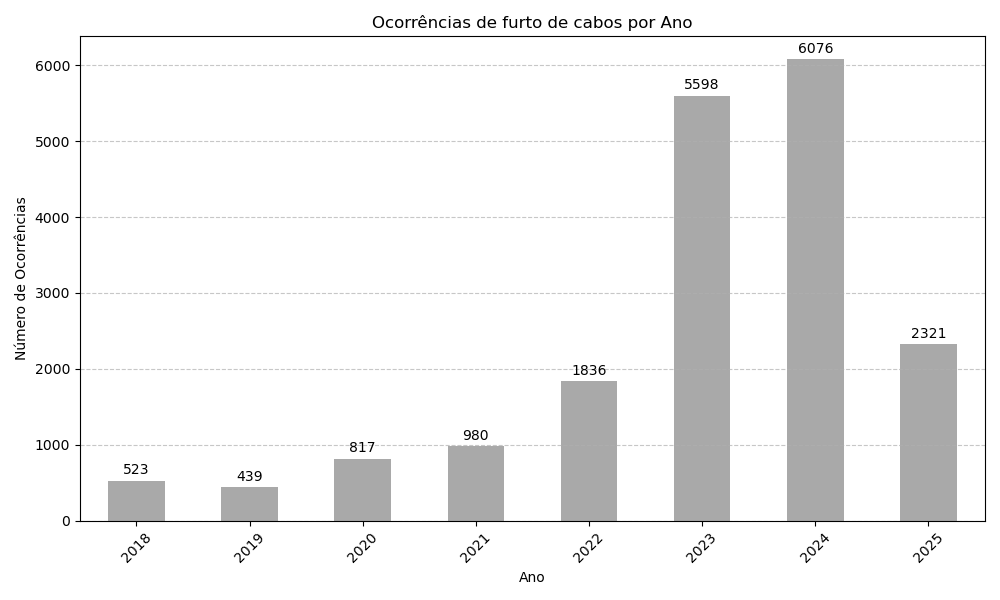
\includegraphics[scale=0.5,keepaspectratio]{dados/images/grafico_barras_ocorrencias_ano.png}
  \caption{Evolução dos eventos de furtos de cabo em Belo Horizonte, no período de 03/2018 a 05/2025.}
  \fonte{Produção própria}
  \label{fig:grafico_barras_ocorrencias_ano}
\end{figure}

Além disso, o simples incremento de novas observações ao conjunto de dados pode ocultar ou impedir a captura de alterações e mudanças, que embora possam parecer sutis, são de fundamental importância para a eficácia da análise, tais como alterações na localização das concentrações do fenômeno e sazonalidades. 

Conforme concluiu Robinson \cite{Robinson1950}, erros podem ser cometidos, ou conclusões equivocadas podem ser obtidas ao se inferir comportamentos individuais a partir de estatísticas de dados agregados, a chamada ``falácia ecológica'' (\textit{``Ecological Fallacy''}). Seu estudo estabeleceu formalmente o problema, mostrando como correlações em nível de grupo (estados, cidades, por exemplo) podem ser completamente diferentes ou até opostas às correlações em nível individual.

Por sua vez, Weisburd \cite{Weisburd2015} complementou este entendimento, ao argumentar pela necessidade de ir além da análise de dados agregados, e buscar padrões espaciais por meio de \textit{hotspots}, ou pontos quentes, onde há concentração de crimes. 

Acrescenta-se, ainda, o efeito de deslocamento geográfico (\textit{``displacement''}) conceituado por Barr \cite{Barr1990}, que explorou as diferentes formas como o crime se move em resposta a ações de prevenção. As figuras apresentadas na Tabela \ref{tab:tabela_mapas} representam, empiricamente, esse deslocamento espacial dos eventos de furto de cabo em Belo Horizonte, além de indicar as diferentes concentrações dos eventos no tempo. Para fins deste comparativo foram considerados apenas os anos de 2023 e 2024, por serem os anos em que há maior volume de dados no dataset.

\begin{table}[htbp]
  \centering
  \begin{tabular}{|m{3.5cm}|m{3.5cm}|m{3.5cm}|m{3.5cm}|}
    \hline
      \begin{minipage}{\linewidth}
        \centering
        \includegraphics[width=3.5cm]{dados/images/mapa_20231_2.png}
        \captionof{figure}{1T 2023}
      \end{minipage}
      &
      \begin{minipage}{\linewidth}
        \centering
        \includegraphics[width=3.5cm]{dados/images/mapa_20232_2.png}
        \captionof{figure}{2T 2023}
      \end{minipage}
      &
      \begin{minipage}{\linewidth}
        \centering
        \includegraphics[width=3.5cm]{dados/images/mapa_20233_2.png}
        \captionof{figure}{3T 2023}
      \end{minipage}
      &
      \begin{minipage}{\linewidth}
        \centering
        \includegraphics[width=3.5cm]{dados/images/mapa_20234_2.png}
        \captionof{figure}{4T 2023}
      \end{minipage}
    \\ \hline
      \begin{minipage}{\linewidth}
        \centering
        \includegraphics[width=3.5cm]{dados/images/mapa_20241_2.png}
        \captionof{figure}{1T 2024}
      \end{minipage}
      &
      \begin{minipage}{\linewidth}
        \centering
        \includegraphics[width=3.5cm]{dados/images/mapa_20242_2.png}
        \captionof{figure}{2T 2024}
      \end{minipage}
      &
      \begin{minipage}{\linewidth}
        \centering
        \includegraphics[width=3.5cm]{dados/images/mapa_20243_2.png}
        \captionof{figure}{3T 2024}
      \end{minipage}
      &
      \begin{minipage}{\linewidth}
        \centering
        \includegraphics[width=3.5cm]{dados/images/mapa_20244_2.png}
        \captionof{figure}{4T 2024}
      \end{minipage}
    \\ \hline
  \end{tabular}
  \caption{Comparação dos mapas de calor por densidade de kernel das observações de furtos de cabo em Belo Horizonte, dos anos de 2023 e 2024, por Trimestre.}
  \fonte{Produção própria}
  \label{tab:tabela_mapas}
\end{table}

Estes fatos corroboram o entendimento de que o método atualmente utilizado pelo COP-BH ainda é insuficiente para uma análise adequada do fenômeno, além do fato de ser executado manualmente. Assim, esse trabalho busca propor um novo método de análise, bem como uma ferramenta para automatizar este processo.

\subsection{Relevância do Problema}

A atividade de monitoramento é realizada sob a perspectiva da prevenção e pronta resposta à ocorrência de crimes, e nesse contexto o crime de furto de cabos. Esse crime tem diversas consequências negativas, tanto econômicas quanto sociais.

Do ponto de vista social e comunitário, podemos citar diversos problemas que o furto de cabos proporcionam à população em geral, tais como a interrupção de serviços de água, luz, acesso à Internet, serviços de saúde, e transtornos nos sistemas de tráfego e transporte público da cidade  (\citenum{Cemig}, \citenum{OGlobo}, \citenum{R7}, \citenum{OTempoA}, \citenum{OTempoB} e \citenum{HojeEmDia}).  

Além disso, há também o impacto econômico, pois o restabelecimento destes serviços demanda o gasto com reparos na infraestrutura de rede elétrica, de telefonia ou de dados, seja pela Administração Pública ou por Concessionárias (\citenum{EstadoDeMinasB}). Pequenos comerciantes e prestadores de serviços também sofrem impactos econômicos decorrentes da interrupção destes serviços essenciais ao funcionamento dos seus estabelecimentos (\citenum{OTempoB}).

Por fim, citam-se os riscos à integridade física dos próprios cometedores deste crime estão expostos, pois podem ser eletrocutados ao manipular cabos e fios de alta tensão, sem as devidas proteções, ou sofrer quedas de altura, ao subir em postes sem equipamentos próprios para isso (\citenum{EstadoDeMinas}). 

Portanto, pode-se perceber que o furto de cabos é um problema público importante, causador de diversos transtornos, e que no âmbito do COP-BH é enfrentado por meio do monitoramento por câmeras e correspondente pronta resposta. Neste sentido, ao buscar o aprimoramento da análise de dados em subsídio ao monitoramento inteligente, este trabalho se propõe a contribuir com o enfrentamento ao furto de cabos, que atinge a diversas cidades brasileiras.

\subsection{Justificativa}

O furto de cabos é um problema é reconhecidamente importante e já existem esforços para resolvê-lo. A própria existência de um processo de trabalho no COP-BH que objetiva a elaboração de um roteiro de monitoramento de furtos de cabos já justifica a importância do tema, pois demonstra que a Instituição reconhece o impacto nocivo à cidade, e busca ativamente otimizar a vigilância. 

Contudo, a abordagem atual possui lacunas críticas que limitam sua eficácia. A metodologia atual, baseada na agregação de todo o histórico de dados em um único mapa de calor estático, se mostra vulnerável a falácias estatísticas, como a falácia ecológica. Ao tratar dados de anos diferentes com o mesmo peso, o método mascara tendências recentes, sazonalidades e, crucialmente, o deslocamento geográfico do crime. Conforme o dataset utilizado, um hotspot de 2022 pode não ter relevância para o monitoramento hoje, mas continua influenciando o mapa de calor atual, diluindo a importância de novos focos e enviesando a compreensão da movimentação do crime.

Tal como já demonstrado, o furto de cabos não é estático, ele se adapta às ações de repressão e resposta. Assim, esse trabalho se justifica pela necessidade de que a análise dos dados seja, também, dinâmica e adaptativa. É preciso compreender para onde as concentrações de furto estão se movimentando, e quando são mais intensas.

Portanto, é necessário desenvolver e implementar uma solução aprimorada e automatizada, que preencha as lacunas e insuficiências identificadas a fim de se obter melhores resultados. 

Com isso, espera-se que, além do aperfeiçoamento na prevenção ao furto de cabos, o modelo metodológico e tecnológico proposto poderá ser adaptado para o combate a outros problemas públicos, fortalecendo a atuação do COP-BH, e contribuindo para uma gestão urbana mais inteligente e segura em Belo Horizonte.

\subsection{Desafios do Projeto}

Tem-se como potenciais desafios do projeto:

\begin{itemize}
  \item{Padronização dos dados: tendo em vista as variadas fontes dos dados, a automatização deverá levar em conta a normalização dos dados, principalmente quanto ao georreferenciamento;} 
  \item{Classificação dos dados: a diversidade de fontes de dados pode ensejar, também, formas e padrões diferentes de classificação;}
  \item{Subnotificação dos dados: pode ocorrer que nem todos os registros de furtos de cabos sejam reportados, ou que sejam reportados com dados imprecisos de data e hora do fato e localização;}
  \item{Disponibilidade dos dados: o dinamismo da análise, com sua automatização, pode ser prejudicado se não houver um meio de capturar os dados de forma rápida;}
  \item{Viéses nos dados: pode ser que os dados estejam sendo capturados em maior volume em locais onde há a presença recorrente de agentes, e em locais onde essa presença seja escassa esteja ocorrendo em igual ou maior volume, mas sem o correspondente registro;}
  \item{Insuficiência de dados: variáveis externas, que também podem ter influência no fenômeno, ainda não estão sendo consideradas;}
  \item{Avaliação da efetividade: pode haver dificuldade em determinar se (ou o quanto) o novo método foi, isoladamente, eficaz na redução da observação do fenômeno.}
\end{itemize}

Alguns dos desafios citados poderão ser contornados durante a execução do trabalho, mas outros, somente após algum período de testes e acompanhamento das percepções operacionais do fenômeno.

\subsection{Contribuição}

%-----------------------------------------------------------------------------------------

\section{OBJETIVOS}
\label{sec:objetivos}
% (máximo de 1/2 página)

\subsection{Objetivo Geral}
\label{subsec:objgeral}
% Objetivo Geral--------------------------------------------------------------------------
%-----------------------------------------------------------------------------------------

\subsection{Objetivos Específicos}
\label{subsec:objespc}
% Objetivos Específicos-------------------------------------------------------------------
%-----------------------------------------------------------------------------------------

\section{TRABALHOS CORRELATOS}
\label{sec:estadoarte}
% Estado da Arte--------------------------------------------------------------------------
% (máximo de 2 páginas)
%-----------------------------------------------------------------------------------------

\section{METODOLOGIA/METODOLOGIA DE DESENVOLVIMENTO} % Escolher o nome mais adequado ao trabalho
\label{sec:metodologia}
% Procedimentos Metodológicos/Metodologia-------------------------------------------------
% (máximo de 2 páginas)
%-----------------------------------------------------------------------------------------

\section{CONCLUSÃO/CONSIDERAÇÕES FINAIS} % Escolher o nome mais adequado ao trabalho
\label{sec:conclusao}
% Conclusão/Considerações Finais----------------------------------------------------------
% (máximo de ½ página)
%-----------------------------------------------------------------------------------------

\section{PLANEJAMENTO DO TRABALHO}
\label{sec:planejamento}
% Planejamento do Trabalho----------------------------------------------------------------
% Esta seção não precisa ser editada, apenas edite o quadro 1 armazenada no diretório ".\dados\quadros"
\begin{quadro}[!htb]
    %\centering
    \caption{Cronograma de Atividades.\label{qua:quadro1}}
    \begin{tabular}{|p{4.5cm}|p{0.7cm}|p{0.7cm}|p{0.7cm}|p{0.7cm}|p{0.7cm}|p{0.7cm}|p{0.7cm}|p{0.7cm}|p{0.7cm}|p{0.7cm}|}
        \hline
        \textbf{Atividades} & \textbf{Mar} & \textbf{Abr} & \textbf{Mai} & \textbf{Jun} & \textbf{Jul} & \textbf{Ago} & \textbf{Set} & \textbf{Out} & \textbf{Nov} & \textbf{Dez} \\
        \hline
        \small{1. Revisão dos apontamentos da banca} &   &   &   &   &   &   &   &   &   &  \\
        \hline
        \small{2. Revisão bibliográfica} &   &   &   &   &   &   &   &   &   &  \\
        \hline
	\small{3. Redação do projeto de TCC} &   &   & X & X &   &   &   &   &   &  \\
        \hline
	\small{4. Defesa do projeto de TCC} &   &   &   &   & X &   &   &   &   &  \\
        \hline
	\small{5. Escrita da Monografia de TCC} &   &   &   &   &   & X & X  & X &   &  \\
        \hline
	\small{6. Elaboração da apresentação final} &   &   &   &   &   &   &   & X & X &  \\
        \hline
	\small{7. Defesa final do TCC} &   &   &   &   &   &   &   &   & X &  \\
        \hline
    \end{tabular}
\end{quadro}


\subsection{DA PROPOSTA AO PROJETO}
%-----------------------------------------------------------------------------------------

\section{RECURSOS NECESSÁRIOS}
\label{sec:recursos}
% Recursos Necessários--------------------------------------------------------------------
%-----------------------------------------------------------------------------------------

\section{HORÁRIO DE TRABALHO}
\label{sec:horário}
% Horário de Trabalho---------------------------------------------------------------------
% Esta seção não precisa ser editada, apenas edite o quadro 2 armazenada no diretório ".\dados\quadros"
\begin{quadro}[!htb]
    %\centering
    \caption{Horário de Trabalho.\label{qua:quadro2}}
    \begin{tabular}{|p{2.5cm}|p{1.8cm}|p{1.8cm}|p{1.8cm}|p{1.8cm}|p{1.8cm}|p{1.8cm}|}
        \hline
        \textbf{Horário} & \textbf{Seg} & \textbf{Ter} & \textbf{Qua} & \textbf{Qui} & \textbf{Sex} & \textbf{Sab} \\
        \hline
        \small{07h30 - 08h20} &   &   &   &   &   &   \\
        \hline
        \small{08h20 - 09h10} &   &   &   &   &   &   \\
        \hline
	\small{09h10 - 10h00} &   &   &  &  &   &   \\
        \hline
	\small{10h10 - 11h00} &   &   &   &   &  &   \\
        \hline
	\small{11h00 - 11h50} &   &   &   &   &   & \\
        \hline
	\small{} &   &   &   &   &   & \\
        \hline
	\small{13h00 - 13h50} &   & TCC & Orientaçao & TCC &   & \\
        \hline
	\small{13h50 - 14h40} &   & TCC & TCC &   &   & \\
        \hline
	\small{14h40 - 15h30} &   & TCC & TCC & TCC &   & \\
        \hline
	\small{15h40 - 16h30} &   & TCC & TCC & TCC &   & \\
        \hline
	\small{16h30 - 17h20} &   &   &   &   &   & \\
        \hline
	\small{17h20 - 18h10} &   &   &   &   &   & \\
        \hline
	\small{} &   &   &   &   &   & \\
	\hline
	\small{18h50 - 19h40} &   &   &   &   &   & \\
        \hline
	\small{19h40 - 20h30} &   &   &   &   &   & \\
        \hline
	\small{20h30 - 21h20} &   &   &   &   &   & \\
        \hline
	\small{21h30 - 22h15} &   &   &   &   &   & \\
        \hline
    \end{tabular}
\end{quadro}

%-----------------------------------------------------------------------------------------
                         % Descrição da Proposta

\postextual
% INSERE ELEMENTOS PÓS-TEXTUAIS
% REFERÊNCIAS------------------------------------------------------------------

% Carrega o arquivo "base-referencias.bib" e extrai automaticamente as referências citadas

\bibliography{./base-referencias}{}
\bibliographystyle{abntex2-alf} % Define o estilo ABNT para formatar a lista de referências

% OBSERVAÇÕES------------------------------------------------------------------
% Este arquivo não precisa ser alterado.
           			   % Referências

\end{document}
